\chapter{Technical Solution}
\label{chap:solution}

\section{The Sovrin Network}
%The DLREP function is a collection of functions proposed by \cite{Brands2000}, and used by \cite{Augot2017}. The instance generator outputs a tuple \[(q, g_1, g_2,...,g_l)\]

In the traditional distributed ledger domain we can differentiate between permissioned and permissionless ledgers. Permissionless ledgers have the advantage of theoretically enable truly decentralized networks, but relies on a reward for the participating nodes to incentivise network contributions. This is usually solved with proof-of-work or proof-of-stake, with the former consuming significant amounts of computing power. Permissioned ledgers is less  reliant on rewards, and the nodes are incentivised buy their stake in the network it self, and requires a foundation or administrative body to recruit and manage nodes and node behavior. In addition, permissioned ledgers are in its nature not truly decentralized.

In an Self-Sovereign Identity network neither of these alternatives can be said to be ideal. Identity should be free to create, maintain and revoke - and a network reliant on nodes without a reward system is not likely to stay healthy. A SSI network with a permissioned node system could work well, as many parties with large stakes in the network would benefit from running nodes and keeping the network healthy. On the other hand, identities management are of such importance that leaving control of the network to a foundation or administrative body is likely to raise concerns at least among the most privacy focused individuals.

This paper proposes the use of a DAC based ledger instead of a blockchain. Using a Directed Acyclic Graph instead of a blockchain allows using a premissionless ledger, while still not monetizing the system to incentivise proof-of-work. As described in Section \ref{sec:background_dlt} the proof-of-work can be done on a per transaction basis, by utilizing the registering device's processors when an attribute is created or verified on the ledger. As double spending is not an issue when the ledger is not keeping track of ownership of value, the required proof-of-work can be adjusted to a level that is acceptable for even mobile devices. The security around tangle is no where near as well tested as that of a blockchain, but technologies like IOTA~\cite{IOTA_Whitepaper} and Raiblocks~\cite{Raiblocks_Whitepaper} are still functioning currencies, and IOTA is noteworthy around 10th place on crypto currency marketcap (Spring 2018).


One of the main concerns around a DAC based approach is the succession of transactions. In a regular blockchain, the block number clearly states what order transactions occurred, while in a DAC it can be impossible to determine the order of two transactions with respect to time. This is not as big of a concern for Self-Sovereign Identity where double spending is not an issue. It can pose a challenge when there is a need for revocation, or if an attribute is allowed to be used only a set number of times. But even in this scenario, the solution is arguably sufficient as invalid transactions will be filtered out by the nodes within minutes.

\newpage
The following sub chapters are largely based on the Sovrin network. Among the open source technologies for Self-Sovereign Identities evaluated in~\ref{sec:ssi_systems}, Sovrin with its on-chain storage and un-monetized public ledger stood out as the best base for a decentralized identity management system.

\section{Storage}
Most of the information associated with an identity is stored on the ledger itself. Some information can be stored in other repositories like a private ledger. The connections, each identified with a unique DID (Distributed Identifier, a cryptonym encoded from the public part of a Ed25519 digital signature scheme), are established between two identity owners. In the Sovrin network, there is no clear distinction between users and providers, but all identity owners are regarded as peers. An identity owner can be a person or an organization. The Sovrin network do have \textit{Stweards} and \textit{Trust Anchors}, \textit{Stweards} are the foundations approved validation nodes, while \textit{Trust Anchors} are a identity owner that has sufficient public evidence of their trustworthiness, and are believed to live up to the Sovrin Promise. \textit{Stweards} are not necessary when utilizing a DAC approach for Self-Sovereign Identity networks, and \textit{Trust Anchors} can not be universally defined in a truly decentralized network. 

A claim is a data structure on the network with one more more attributes, and can be made by a identity owner about themselves (unverified) or by another identity owner about a user (verified). Each claim also contains a definition, such that anyone can easily look up the data structure and make sense of the claim.

\section{Enrollment}
In the Sovrin network, anyone can create the Master Secret for an identity account. The first DID registered on the identity is called the Genesis Record, and the network classifies the identity as a Sovrin Identity when the Genesis Record are stored and verified. The network requires the Genesis Record to be verified by a Trust Anchor for a regular identity owner, a factor that increases the trust of a Sovrin Identity, but is impossible to implement in a truly centralized system like a DAC.
\section{Verification}

\section{Attribute Segregation}
For each claim, a unique key pair is used. In addition, claims can be reused and tailored to the purpose using what Sovrin describes as Disclosure proofs. This allows claims to be used without disclosing exess information about the user.
\section{Revocation}

\section{Recovery}

\section{Challenges}
Lack of knowledge, storage capacity 
\begin{figure}[ht]
    \centering
    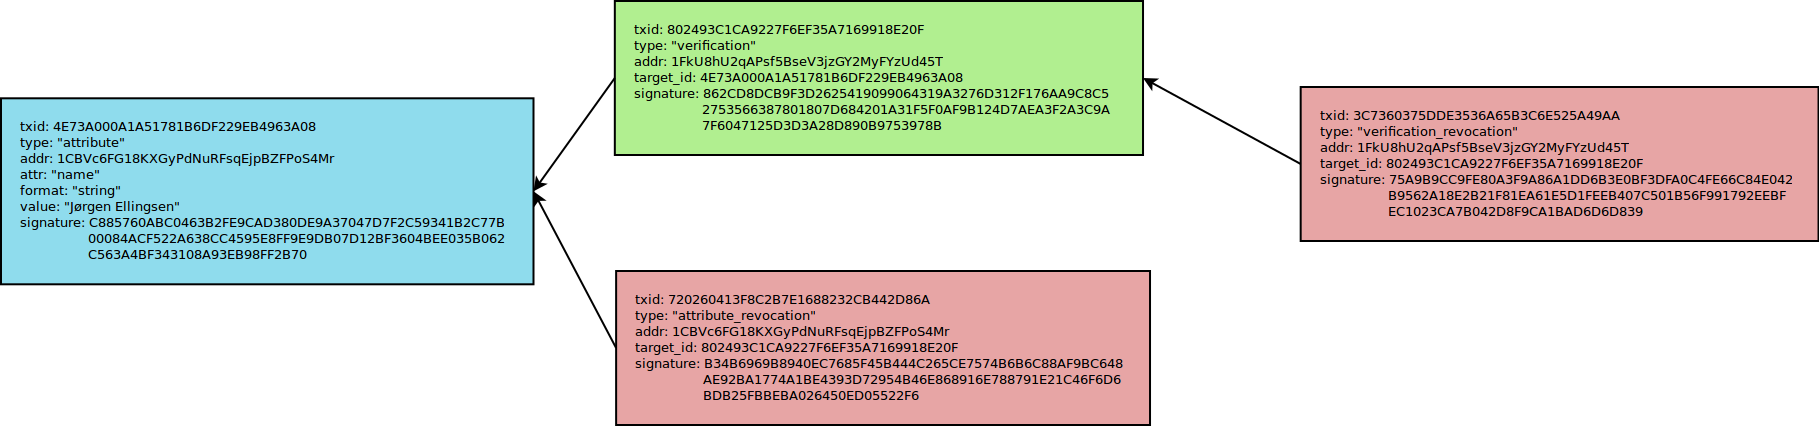
\includegraphics[width=1\textwidth]{DACSigning.png}
    \caption{Verification and Revocation}
    \label{fig:dac_sign}
\end{figure}
